\documentclass[11pt,oneside]{article}
\usepackage[a4paper,margin=27mm,headheight=15pt]{geometry}
\usepackage[T1]{fontenc}
\usepackage[utf8]{inputenc}
\IfFileExists{libertinus.sty}{\usepackage{libertinus}}{\usepackage{lmodern}}
\usepackage{microtype}
\usepackage{amsmath,amssymb,amsthm,mathtools,mathrsfs}
\usepackage{bm}
\usepackage{booktabs,longtable,array,tabularx}
\usepackage{graphicx}
\usepackage{pgfplots}
\usepackage{xcolor}
\usepackage{enumitem}
\usepackage{fancyhdr}
\usepackage{titlesec}
\usepackage{listings}
\usepackage{xurl}
\usepackage{hyperref}
\usepackage[nameinlink,noabbrev]{cleveref}

\definecolor{linkblue}{RGB}{25,75,135}
\definecolor{shadegray}{RGB}{246,247,249}
\definecolor{rulegray}{RGB}{195,201,208}
\pgfplotsset{compat=1.18}
\hypersetup{
  colorlinks=true,
  linkcolor=linkblue,
  citecolor=linkblue,
  urlcolor=linkblue,
  pdftitle={Iterated Thue--Morse Prefix Sums and the Fabius Function},
  pdfsubject={A sharp convergence rate for the corrected prefix approximation},
  pdfkeywords={Fabius function, Rvachev up-function, Thue-Morse, prefix sums, convergence rate, histogram approximation}
}
\pagestyle{fancy}
\fancyhf{}
\fancyhead[L]{\small Fabius--Rvachev synthesis}
\fancyhead[R]{\small\nouppercase{\leftmark}}
\fancyfoot[C]{\thepage}
\renewcommand{\headrulewidth}{0.4pt}
\titleformat{\section}{\Large\bfseries}{\thesection}{0.7em}{}
\titleformat{\subsection}{\large\bfseries}{\thesubsection}{0.7em}{}
\titleformat{\subsubsection}{\normalsize\bfseries}{\thesubsubsection}{0.7em}{}
\setcounter{secnumdepth}{3}
\setcounter{tocdepth}{2}
\setlist[itemize]{leftmargin=2em,itemsep=0.25em,topsep=0.4em}
\setlist[enumerate]{leftmargin=2.3em,itemsep=0.25em,topsep=0.4em}
\setlength{\emergencystretch}{2em}

\newtheorem{theorem}{Theorem}[section]
\newtheorem{proposition}[theorem]{Proposition}
\newtheorem{lemma}[theorem]{Lemma}
\newtheorem{corollary}[theorem]{Corollary}
\newtheorem{conjecture}[theorem]{Conjecture}
\theoremstyle{definition}
\newtheorem{definition}[theorem]{Definition}
\newtheorem{algorithm}[theorem]{Algorithm}
\newtheorem{example}[theorem]{Example}
\theoremstyle{remark}
\newtheorem{remark}[theorem]{Remark}
\newtheorem{warning}[theorem]{Warning}

\newcommand{\R}{\mathbb R}
\newcommand{\C}{\mathbb C}
\newcommand{\Q}{\mathbb Q}
\newcommand{\N}{\mathbb N}
\newcommand{\Z}{\mathbb Z}
\newcommand{\Up}{\operatorname{up}}
\newcommand{\sinc}{\operatorname{sinc}}
\newcommand{\wt}{\operatorname{wt}_2}
\newcommand{\e}{\mathrm e}
\newcommand{\ii}{\mathrm i}
\newcommand{\dd}{\,\mathrm d}
\newcommand{\Var}{\operatorname{Var}}
\newcommand{\E}{\mathbb E}
\newcommand{\Prob}{\mathbb P}
\newcommand{\bigO}{\mathcal O}
\newcommand{\smallo}{o}
\newcommand{\supp}{\operatorname{supp}}
\newcommand{\repo}{\nolinkurl{Analysis/FabiusFunction}}
\newcommand{\norm}[1]{\left\lVert #1\right\rVert}
\newcommand{\abs}[1]{\left\lvert #1\right\rvert}
\newcommand{\floor}[1]{\left\lfloor #1\right\rfloor}
\newcommand{\fracpart}[1]{\left\{#1\right\}}
\newcommand{\Btri}[1]{\binom{#1}{2}}
\newcommand{\indicator}{\mathbf 1}

\newenvironment{proofidea}{\par\smallskip\noindent\textit{Proof architecture.}\ }{\hfill$\square$\par\smallskip}
\newenvironment{boxedremark}{%
  \par\smallskip\noindent\begin{center}\begin{minipage}{0.94\textwidth}%
  \color{black}\hrule\vspace{0.6em}\small
}{%
  \vspace{0.6em}\hrule\end{minipage}\end{center}\smallskip
}
\lstdefinestyle{pseudo}{
  basicstyle=\ttfamily\small,
  backgroundcolor=\color{shadegray},
  frame=single,
  rulecolor=\color{rulegray},
  columns=fullflexible,
  keepspaces=true,
  showstringspaces=false,
  xleftmargin=0.7em,
  xrightmargin=0.7em,
  aboveskip=0.8em,
  belowskip=0.8em
}

\title{\bfseries Iterated Thue--Morse Prefix Sums and the Fabius Function\\[0.35em]
\large Exact centering, a sharp $n2^{-n}$ law, and faster recentered approximations}
\author{A complementary report to the Fabius--Rvachev synthesis\\
\small Based on Vladimir Reshetnikov's \texttt{ProveIt} formal development}
\date{Repository snapshot studied: 25 August 2026}

\begin{document}
\maketitle

\begin{abstract}
Let $\varepsilon_m=(-1)^{\wt(m)}$ be the signed Thue--Morse sequence and let
$\sigma_{k+1}(m)=\sum_{j=0}^{m}\sigma_k(j)$ be its iterated \emph{inclusive}
prefix sums.  The formal development in the \texttt{ProveIt} repository proves
that
\[
 \mathcal A_n(x)=
 \frac{\sigma_{n+1}(\floor{2^n x})}{2^{\binom n2}},
 \qquad 0\le x\le1,
\]
converges pointwise to the bounded Fabius function $F(x)$.  The existing
exposition deliberately asserts no rate.  This report supplies one.

The coefficient carrying $\mathcal A_n(x)$ is the value of a polynomial
histogram at a cell center, but that center is not $x-1$.  Its exact displacement is
\[
 \delta_n(x)=\frac{n+2-2\fracpart{2^n x}}{2^{n+1}}
 =\frac{n}{2^{n+1}}+\frac{1-\fracpart{2^n x}}{2^n}.
\]
At the histogram centers themselves, a Fourier-tail factorization and a cardinal
moment calculation give the uniform estimate
\[
 \abs{\mathcal W_n(\xi_{n,m})-\Up(\xi_{n,m})}
 \le \left(\frac{4n}{3}+\frac{16}{9}\right)4^{-n}.
\]
Consequently, uniformly for $x\in[0,1]$ and $n\ge3$,
\[
 \mathcal A_n(x)=F(x)+F'(x)\delta_n(x)
 +\frac12F''(x)\delta_n(x)^2+\rho_n(x),
\]
where
\[
 \abs{\rho_n(x)}\le
 \left(\frac{4n}{3}+\frac{16}{9}\right)4^{-n}
 +\frac43(n+2)^3 8^{-n}.
\]
In fact the entire normalized error profile converges uniformly:
\[
 \frac{2^n}{n}\bigl(\mathcal A_n-F\bigr)
 \longrightarrow \frac12F'
 \qquad\text{in }L^\infty[0,1].
\]
Consequently the uniform error has the sharp constant
\[
 \boxed{\displaystyle
 \lim_{n\to\infty}\frac{2^n}{n}
 \norm{\mathcal A_n-F}_{L^\infty[0,1]}=1.}
\]
The factor $n$ is therefore not an intrinsic weakness of the Thue--Morse
coefficients.  It is a deterministic centering drift.  The histogram itself has
uniform error asymptotic to $2^{-n}$, while linear interpolation through the
correct coefficient centers has the explicit faster bound $\bigl(4n/3+25/9\bigr)4^{-n}$.
The report also records exact endpoint and midpoint formulas, a three-scale
asymptotic expansion containing the binary phase $\fracpart{2^n x}$, and a roadmap
for formalizing the new quantitative theorem in Lean.
\end{abstract}

\tableofcontents
\newpage

\section{Scope, conventions, and the quantitative question}
\label{sec:scope}

The purpose of this report is narrow but structurally revealing.  The existing
Fabius--Rvachev synthesis develops the discrete Thue--Morse construction in full:
the prefix hierarchy, its binomial convolution kernel, the dyadic zero runs, the
formal generating series, the corrected normalization, the exact identification
with the polynomial histogram, and the resulting pointwise convergence
\cite{proveit,synthesis}.  The corresponding Lean module
\path{ThueMorseApproximation.lean} explicitly says that no quantitative uniform
rate is asserted.  We keep every convention of that development and add the
missing estimate.

Throughout, $F$ is the bounded Fabius distribution function, equal to $0$ on
$(-\infty,0]$ and to $1$ on $[1,\infty)$, and $\Up$ is Rvachev's even compactly
supported bump,
\begin{equation}
 \Up(y)=F(1-|y|),\qquad
 F(x)=\Up(x-1)\quad(0\le x\le1).                 \label{eq:fold}
\end{equation}
We use the Fourier transform
\begin{equation}
 \widehat f(\xi)=\int_{\R}f(x)\e^{-2\pi\ii x\xi}\dd x,
 \qquad \sinc z=\frac{\sin z}{z}.               \label{eq:fourier-convention}
\end{equation}
The derivative bounds proved sharply in the formal development are
\begin{equation}
 \norm{F^{(r)}}_\infty\le 2^{\binom{r+1}{2}},
 \qquad
 \norm{\Up^{(r)}}_\infty\le 2^{\binom{r+1}{2}}.  \label{eq:derivative-bounds}
\end{equation}
We shall use, in particular,
\begin{equation}
 0\le F'\le2,
 \qquad \norm{F''}_\infty\le8,
 \qquad \norm{F'''}_\infty\le64,                \label{eq:low-derivative-bounds}
\end{equation}
and $F'(1/2)=2$.

The central question is not merely whether the prefix sequence converges, but
which of three mechanisms controls its error:
\begin{enumerate}
\item the difference between the finite coefficient histogram and $\Up$ at the
      exact coefficient centers;
\item the discretization incurred by replacing a smooth function with a step
      histogram;
\item the displacement between the center selected by the published floor index
      and the intended evaluation point.
\end{enumerate}
The answer is unexpectedly clean.  These effects have orders
$ n4^{-n}$, $2^{-n}$, and $n2^{-n}$, respectively.  The third dominates the
particular floor-sampled approximation to $F$.

\begin{boxedremark}
\textbf{Status of formal verification.}
The exact prefix--coefficient identity and the qualitative convergence used here
are already formalized in Lean.  The quantitative center estimate, the asymptotic
expansion, and the sharp constant $1$ are new deductions in this report.  They
are presented with complete conventional proofs, but they have not been added to
the repository's Lean files as of the snapshot date.
\end{boxedremark}

\section{The discrete hierarchy}
\label{sec:discrete}

\subsection{Signed Thue--Morse and inclusive summation}

Let
\begin{equation}
 \varepsilon_m=(-1)^{\wt(m)},                              \label{eq:tm-sign}
\end{equation}
where $\wt(m)$ is the number of $1$'s in the binary expansion of $m$.  Define
\begin{equation}
 \sigma_0(m)=\varepsilon_m,
 \qquad
 \sigma_{k+1}(m)=\sum_{j=0}^{m}\sigma_k(j).                \label{eq:prefix-def}
\end{equation}
The summation is inclusive.  Thus
\begin{equation}
 \sigma_{k+1}(m+1)-\sigma_{k+1}(m)=\sigma_k(m+1),           \label{eq:forward-difference}
\end{equation}
with the lower-order value evaluated at the new index.  This one-place shift is
responsible for the order correction that appears later.

Repeated summation gives the discrete B-spline convolution law
\begin{equation}
 \sigma_k(m)=\sum_{r=0}^{m}
 \binom{m-r+k-1}{k-1}\varepsilon_r,
 \qquad k\ge1.                                             \label{eq:binomial-convolution}
\end{equation}
Equivalently,
\begin{equation}
 \sigma_{k+1}(m)=\sum_{r=0}^{m}
 \binom{m-r+k}{k}\varepsilon_r.                            \label{eq:binomial-convolution-shift}
\end{equation}
The kernel is the coefficient sequence of $(1-z)^{-k}$.

The formal generating functions make the same statement in one line.  On the
first dyadic block,
\begin{equation}
 K_r(z)=\sum_{m=0}^{2^r-1}\varepsilon_m z^m
       =\prod_{j=0}^{r-1}(1-z^{2^j}),                      \label{eq:tm-block-product}
\end{equation}
and coefficientwise the infinite signed series is
\begin{equation}
 K(z)=\prod_{j\ge0}(1-z^{2^j}).                            \label{eq:tm-infinite-product}
\end{equation}
Hence the $k$-fold prefix series is formally
\begin{equation}
 S_k(z)=\sum_{m\ge0}\sigma_k(m)z^m=\frac{K(z)}{(1-z)^k}.  \label{eq:prefix-series}
\end{equation}
No analytic convergence is involved in this identity.

\subsection{Dyadic annihilation}

The product in \eqref{eq:tm-block-product} has a zero of order $r$ at $z=1$.
Equivalently, a complete block of length $2^r$ annihilates every polynomial in
$m$ of degree below $r$.  Applied to \eqref{eq:binomial-convolution}, this gives
the exact zero run
\begin{equation}
 \sigma_k(m)=0
 \quad\text{for}\quad
 2^r-k\le m\le2^r-1,
 \qquad 1\le k\le r,                                     \label{eq:zero-run}
\end{equation}
with sharp boundary values
\begin{equation}
 \sigma_k(2^r-k-1)=(-1)^{r-k},
 \qquad
 \sigma_k(2^r)=-1.                                        \label{eq:zero-run-boundary}
\end{equation}
These identities explain both the long flat regions of the iterated prefixes and
the exceptional right endpoint of the unit-interval grid.

\section{The exact polynomial bridge}
\label{sec:polynomial-bridge}

\subsection{Approximation polynomials}

Put
\begin{equation}
 P_n(z)=\prod_{j=1}^{n}(1+z+\cdots+z^{2^j-1})
       =\sum_{m=0}^{g_n}a_{n,m}z^m,                        \label{eq:Pn}
\end{equation}
with $P_0=1$.  Its degree and total mass are
\begin{equation}
 g_n=\sum_{j=1}^{n}(2^j-1)=2^{n+1}-n-2,
 \qquad
 P_n(1)=2^{\binom{n+1}{2}}.                                \label{eq:degree-mass}
\end{equation}
The coefficients count restricted sums
\begin{equation}
 a_{n,m}=
 \#\left\{(s_1,\ldots,s_n):
 0\le s_j<2^j,\ \sum_{j=1}^{n}s_j=m\right\}.              \label{eq:coefficient-count}
\end{equation}
They are nonnegative and symmetric: $a_{n,m}=a_{n,g_n-m}$.

The denominator-cleared product identity is
\begin{equation}
 (1-z)^{n+1}P_n(z)=\prod_{j=0}^{n}(1-z^{2^j}).              \label{eq:cleared-product}
\end{equation}
Comparing \eqref{eq:cleared-product} with
\eqref{eq:prefix-series} gives the exact coefficient bridge
\begin{equation}
 \boxed{\displaystyle
 \sigma_{n+1}(m)=a_{n,m}
 \quad\text{whenever}\quad 0\le m<2^{n+1}.}               \label{eq:prefix-coefficient}
\end{equation}
The restriction is real: at $m=2^{n+1}$ the left side is $-1$ by
\eqref{eq:zero-run-boundary}, while the polynomial coefficient is zero.

\subsection{The centered probability measure and histogram}

Let
\begin{equation}
 h_n=2^{-n},
 \qquad
 \xi_{n,m}=\frac{2m-g_n}{2^{n+1}}
          =h_n\left(m-\frac{g_n}{2}\right).                \label{eq:centers}
\end{equation}
The centers form an arithmetic progression of mesh $h_n$.  Define the atomic
probability measure
\begin{equation}
 \mu_n=\sum_{m\in\Z}p_{n,m}\,\delta_{\xi_{n,m}},
 \qquad
 p_{n,m}=\frac{a_{n,m}}{2^{\binom{n+1}{2}}},               \label{eq:mu-n}
\end{equation}
where $a_{n,m}=0$ outside $0\le m\le g_n$.  Let
\begin{equation}
 \beta_h(x)=\frac1h\indicator_{[-h/2,h/2]}(x)              \label{eq:box-density}
\end{equation}
with the harmless half-weight convention at the two endpoints.  The polynomial
histogram is
\begin{equation}
 \mathcal W_n=\mu_n*\beta_{h_n}.                            \label{eq:histogram-convolution}
\end{equation}
At a center only its own atom contributes, and therefore
\begin{equation}
 \mathcal W_n(\xi_{n,m})
 =\frac{p_{n,m}}{h_n}
 =\frac{a_{n,m}}{2^{\binom n2}}.                           \label{eq:center-value}
\end{equation}
Combining \eqref{eq:prefix-coefficient} and \eqref{eq:center-value} yields the
formalized exact identification
\begin{equation}
 \frac{\sigma_{n+1}(m)}{2^{\binom n2}}
 =\mathcal W_n(\xi_{n,m}),
 \qquad 0\le m<2^{n+1}.                                   \label{eq:exact-grid-histogram}
\end{equation}

\section{What the floor index actually samples}
\label{sec:centering}

The corrected prefix sample for the bump is
\begin{equation}
 \mathcal J_n(t)=
 \frac{\sigma_{n+1}(\floor{2^{n+1}t})}{2^{\binom n2}},
 \qquad 0\le t\le1.                                      \label{eq:J-def}
\end{equation}
For $t<1$, \eqref{eq:exact-grid-histogram} gives
\begin{equation}
 \mathcal J_n(t)=
 \mathcal W_n\!\left(\xi_{n,\floor{2^{n+1}t}}\right).    \label{eq:J-histogram}
\end{equation}
The Fabius version is the first-half rescaling
\begin{equation}
 \mathcal A_n(x)=\mathcal J_n(x/2)
 =\frac{\sigma_{n+1}(\floor{2^n x})}{2^{\binom n2}},
 \qquad 0\le x\le1.                                     \label{eq:A-def}
\end{equation}

\begin{lemma}[Exact center drift]
\label{lem:center-drift}
For $x\in[0,1]$, put
\begin{equation}
 \theta_n(x)=\fracpart{2^n x},
 \qquad
 \delta_n(x)=\frac{n+2-2\theta_n(x)}{2^{n+1}}.            \label{eq:delta-def}
\end{equation}
Then
\begin{equation}
 \xi_{n,\floor{2^n x}}=x-1+\delta_n(x),                   \label{eq:center-drift}
\end{equation}
and
\begin{equation}
 \delta_n(x)=\frac{n}{2^{n+1}}+
              \frac{1-\theta_n(x)}{2^n},
 \qquad
 \frac{n}{2^{n+1}}<\delta_n(x)\le\frac{n+2}{2^{n+1}}.    \label{eq:delta-decompose}
\end{equation}
\end{lemma}

\begin{proof}
Use $g_n=2^{n+1}-n-2$ and
$\floor{2^n x}=2^n x-\theta_n(x)$ in \eqref{eq:centers}:
\begin{align*}
 \xi_{n,\floor{2^n x}}
 &=\frac{2(2^n x-\theta_n(x))-(2^{n+1}-n-2)}{2^{n+1}}\\
 &=x-1+\frac{n+2-2\theta_n(x)}{2^{n+1}}.
\end{align*}
The decomposition and bounds follow from $0\le\theta_n(x)<1$.
\end{proof}

The dominant term in \eqref{eq:delta-decompose} is $n2^{-n-1}$.  It comes from
the deficit $n+2$ in the degree $g_n=2^{n+1}-n-2$, not from random rounding.
The binary fractional part contributes the lower-order oscillation
$(1-\theta_n(x))2^{-n}$.

\begin{boxedremark}
\textbf{The source of the rate.}
The approximation does not read the histogram near $x-1$ and then incur a
single-cell error.  It reads a center roughly $n/2$ cells to the right.  Since
$F'$ is generally nonzero, a smooth function changes by order
$(n/2)h_n=n2^{-n-1}$ across that displacement.  Any proof that ignores the exact
center formula can at best obscure this leading term.
\end{boxedremark}

\section{Fourier factorization of the omitted tail}
\label{sec:tail-kernel}

\subsection{The cosine products}

The centered uniform variable on the $2^j$ lattice points of spacing $h_n$ has
Fourier transform
\begin{equation}
 \frac{\sin(\pi 2^j h_n\xi)}{2^j\sin(\pi h_n\xi)}
 =\prod_{r=0}^{j-1}\cos(\pi 2^r h_n\xi).                  \label{eq:finite-uniform-transform}
\end{equation}
Multiplying over $j=1,\ldots,n$ and collecting equal cosine factors gives
\begin{equation}
 \widehat\mu_n(\xi)
 =\prod_{\ell=1}^{n}
   \cos\!\left(\frac{\pi\xi}{2^\ell}\right)^\ell.       \label{eq:mu-cosine-product}
\end{equation}
The Rvachev bump has the infinite product
\begin{equation}
 \widehat\Up(\xi)
 =\prod_{\ell=1}^{\infty}
   \cos\!\left(\frac{\pi\xi}{2^\ell}\right)^\ell.      \label{eq:up-cosine-product}
\end{equation}
This is equivalent to the more familiar infinite sinc product.

Set $h=h_n$.  Reindexing the tail of \eqref{eq:up-cosine-product} gives
\begin{align}
 \prod_{\ell=n+1}^{\infty}
 \cos\!\left(\frac{\pi\xi}{2^\ell}\right)^\ell
 &=\prod_{r=1}^{\infty}
   \cos\!\left(\frac{\pi h\xi}{2^r}\right)^{n+r} \notag\\
 &=\widehat\Up(h\xi)
   \left(\prod_{r=1}^{\infty}
     \cos\!\left(\frac{\pi h\xi}{2^r}\right)\right)^n \notag\\
 &=\widehat\Up(h\xi)\sinc(\pi h\xi)^n.                  \label{eq:tail-factorization}
\end{align}
In the last line we used
$\prod_{r\ge1}\cos(z/2^r)=\sin z/z$.

Let $D_h\Up(x)=h^{-1}\Up(x/h)$ and define the tail density
\begin{equation}
 q_n=\beta_h^{*n}*D_h\Up.                                  \label{eq:q-n}
\end{equation}
The Fourier identity \eqref{eq:tail-factorization} is precisely
\begin{equation}
 \boxed{\Up=\mu_n*q_n.}                                    \label{eq:up-mu-q}
\end{equation}
Thus the limit is obtained from the discrete polynomial law by adding $n$
independent uniform jitters of width $h$ and an independent scaled copy of the
whole Rvachev law.

\subsection{A cardinal probability distribution}

At the mesh points define
\begin{equation}
 \lambda_{n,k}=h q_n(kh),\qquad k\in\Z.                    \label{eq:lambda-def}
\end{equation}
The $\lambda_{n,k}$ form a symmetric probability distribution on $\Z$.
Indeed, write $q_n=\beta_h*\rho_n$.  Since translates of the box tile the line,
\begin{equation}
 h\sum_{k\in\Z}\beta_h(kh-s)=1                            \label{eq:box-partition}
\end{equation}
for almost every $s$.  Integration against $\rho_n$ yields
\begin{equation}
 \sum_{k\in\Z}\lambda_{n,k}=1,
 \qquad \lambda_{n,-k}=\lambda_{n,k}.                     \label{eq:lambda-probability}
\end{equation}
Equation \eqref{eq:up-mu-q}, together with
$p_{n,m}=h\mathcal W_n(\xi_{n,m})$, now becomes the exact cardinal averaging
identity
\begin{equation}
 \Up(\xi_{n,m})=
 \sum_{k\in\Z}\lambda_{n,k}
 \mathcal W_n(\xi_{n,m-k}).                               \label{eq:cardinal-average}
\end{equation}
The value of the smooth limit at a center is therefore a symmetric local average
of the neighboring coefficient heights.

The second moment of this discrete averaging law is also exact.

\begin{lemma}[Cardinal second moment]
\label{lem:cardinal-second-moment}
For $n\ge3$,
\begin{equation}
 \sum_{k\in\Z}k^2\lambda_{n,k}
 =\frac{n}{12}+\frac19.                                   \label{eq:lambda-second-moment}
\end{equation}
\end{lemma}

\begin{proof}
After scaling by $h$, let
\begin{equation*}
 \kappa_n=\beta_1^{*n}*\Up,
 \qquad \lambda_{n,k}=\kappa_n(k).
\end{equation*}
Its Fourier transform is
$\widehat\kappa_n(\xi)=\sinc(\pi\xi)^n\widehat\Up(\xi)$.
Poisson summation, differentiated twice, gives
\begin{equation*}
 -4\pi^2\sum_{k\in\Z}k^2\kappa_n(k)
 =\sum_{j\in\Z}\widehat\kappa_n''(j).
\end{equation*}
At every nonzero integer $j$, the factor $\sinc(\pi\xi)^n$ has a zero of order
$n\ge3$, so the second derivative vanishes there.  Only $j=0$ remains, and hence
the discrete second moment equals the ordinary second moment of $\kappa_n$.

The variance of a uniform variable on $[-1/2,1/2]$ is $1/12$.  The cosine
product \eqref{eq:up-cosine-product} represents the Rvachev law as the sum of
$\ell$ independent signs of amplitude $2^{-\ell-1}$ at every level $\ell$;
therefore
\begin{equation*}
 \Var(\Up)=\sum_{\ell=1}^{\infty}
 \frac{\ell}{2^{2\ell+2}}
 =\frac14\sum_{\ell=1}^{\infty}\ell4^{-\ell}
 =\frac19.
\end{equation*}
Variances add under convolution, giving \eqref{eq:lambda-second-moment}.
\end{proof}

\section{Discrete curvature of the coefficient rows}
\label{sec:curvature}

Write
\begin{equation}
 w_{n,m}=\frac{a_{n,m}}{2^{\binom n2}},                    \label{eq:w-def}
\end{equation}
with $w_{n,m}=0$ outside the polynomial support.  Thus
$w_{n,m}=\mathcal W_n(\xi_{n,m})$.

We first need a uniform coefficient bound.  The recurrence
\begin{equation}
 P_r(z)=P_{r-1}(z)(1+z+\cdots+z^{2^r-1})                  \label{eq:P-recursion}
\end{equation}
shows that every coefficient of $P_r$ is a partial sum of coefficients of
$P_{r-1}$.  Consequently
\begin{equation}
 0\le a_{r,m}\le P_{r-1}(1)=2^{\binom r2}.                 \label{eq:coefficient-max}
\end{equation}
Equality holds on the central plateau
$g_{r-1}\le m\le2^r-1$.

The relevant smoothness is measured by the second finite difference.

\begin{lemma}[Uniform discrete curvature]
\label{lem:discrete-curvature}
For $n\ge3$ and every $m\in\Z$,
\begin{equation}
 \abs{w_{n,m}-2w_{n,m-1}+w_{n,m-2}}
 \le 32\,4^{-n}.                                          \label{eq:curvature-bound}
\end{equation}
\end{lemma}

\begin{proof}
Factor off the last two geometric polynomials:
\begin{equation}
 (1-z)^2P_n(z)
 =(1-z^{2^{n-1}})(1-z^{2^n})P_{n-2}(z).                   \label{eq:second-difference-product}
\end{equation}
The coefficient on the left is
$a_{n,m}-2a_{n,m-1}+a_{n,m-2}$.  The coefficient on the right is a signed sum
of four coefficients of $P_{n-2}$.  By \eqref{eq:coefficient-max}, each has
absolute value at most $2^{\binom{n-2}{2}}$.  Division by
$2^{\binom n2}$ gives
\begin{equation*}
 4\,2^{\binom{n-2}{2}-\binom n2}
 =4\,2^{-(2n-3)}=32\,4^{-n}.
\end{equation*}
\end{proof}

\begin{lemma}[Symmetric discrete Taylor bound]
\label{lem:symmetric-discrete-taylor}
If a doubly infinite sequence $(v_m)$ satisfies
$\abs{v_m-2v_{m-1}+v_{m-2}}\le M$ for all $m$, then
\begin{equation}
 \abs{v_{m+k}+v_{m-k}-2v_m}\le Mk^2
 \qquad(k\ge0).                                           \label{eq:symmetric-second-difference}
\end{equation}
\end{lemma}

\begin{proof}
Let $d_m=v_m-v_{m-1}$.  Consecutive first differences satisfy
$\abs{d_m-d_{m-1}}\le M$.  Expanding the two increments from $m$ to $m+k$ and
from $m-k$ to $m$, and pairing their first differences, yields a sum of
$1+3+\cdots+(2k-1)=k^2$ second differences.
\end{proof}

\section{The intrinsic error at coefficient centers}
\label{sec:center-error}

We can now quantify the part of the approximation that the qualitative moving
argument proof leaves hidden.

\begin{theorem}[Uniform center estimate]
\label{thm:center-estimate}
For every $n\ge3$ and every $m\in\Z$,
\begin{equation}
 \boxed{\displaystyle
 \abs{\mathcal W_n(\xi_{n,m})-\Up(\xi_{n,m})}
 \le
 \left(\frac{4n}{3}+\frac{16}{9}\right)4^{-n}.}            \label{eq:center-estimate}
\end{equation}
\end{theorem}

\begin{proof}
Use \eqref{eq:cardinal-average}, symmetry of $\lambda_{n,k}$, and
$\sum_k\lambda_{n,k}=1$:
\begin{align*}
 \Up(\xi_{n,m})-w_{n,m}
 &=\sum_{k\ge1}\lambda_{n,k}
   \bigl(w_{n,m+k}+w_{n,m-k}-2w_{n,m}\bigr).
\end{align*}
By \cref{lem:discrete-curvature,lem:symmetric-discrete-taylor}, the absolute
value of the bracket is at most $32\,4^{-n}k^2$.  Therefore
\begin{align*}
 \abs{\Up(\xi_{n,m})-w_{n,m}}
 &\le32\,4^{-n}\sum_{k\ge1}k^2\lambda_{n,k}\\
 &=16\,4^{-n}\sum_{k\in\Z}k^2\lambda_{n,k}\\
 &=16\,4^{-n}\left(\frac{n}{12}+\frac19\right),
\end{align*}
which is \eqref{eq:center-estimate}.
\end{proof}

The proof separates two independent facts.  The coefficient row has curvature
$\bigO(4^{-n})$ per lattice step, while the omitted Fourier tail averages over a
discrete variance of order $n$.  Their product is $\bigO(n4^{-n})$.

\begin{remark}[An elementary but weaker constant]
If one avoids the Poisson calculation in \cref{lem:cardinal-second-moment}, the
support of $q_n$ gives $\lambda_{n,k}=0$ for
$\abs{k}>(n+2)/2$.  The same argument then yields
\begin{equation*}
 \abs{\mathcal W_n(\xi_{n,m})-\Up(\xi_{n,m})}
 \le4(n+2)^2 4^{-n}.
\end{equation*}
This already suffices for the sharp $n2^{-n}$ law.  The cardinal moment is what
improves the intrinsic estimate from $\bigO(n^2 4^{-n})$ to
$\bigO(n4^{-n})$.
\end{remark}

\section{The sharp expansion for the Fabius sample}
\label{sec:main-rate}

We now combine the exact drift with the center estimate.  Recall
$\mathcal A_n$ from \eqref{eq:A-def} and $\delta_n$ from \eqref{eq:delta-def}.

\begin{theorem}[Uniform second-order expansion]
\label{thm:second-order-expansion}
For every $n\ge3$ and every $x\in[0,1]$,
\begin{equation}
 \boxed{\displaystyle
 \mathcal A_n(x)
 =F(x)+F'(x)\delta_n(x)
 +\frac12F''(x)\delta_n(x)^2+\rho_n(x),}                   \label{eq:second-order-expansion}
\end{equation}
where
\begin{equation}
 \abs{\rho_n(x)}\le
 \left(\frac{4n}{3}+\frac{16}{9}\right)4^{-n}
 +\frac43(n+2)^3 8^{-n}.                                  \label{eq:second-order-remainder}
\end{equation}
\end{theorem}

\begin{proof}
Put $m=\floor{2^n x}$ and $y=x-1$.  Since $m<2^{n+1}$,
\eqref{eq:exact-grid-histogram} and \cref{lem:center-drift} give
\begin{equation*}
 \mathcal A_n(x)=\mathcal W_n(\xi_{n,m}),
 \qquad
 \xi_{n,m}=y+\delta_n(x).
\end{equation*}
By \cref{thm:center-estimate}, replacing $\mathcal W_n$ by $\Up$ at this center
costs at most $(4n/3+16/9)4^{-n}$.  Taylor's theorem and
$\norm{\Up'''}_\infty\le64$ give
\begin{equation*}
 \Up(y+\delta)=\Up(y)+\Up'(y)\delta+\frac12\Up''(y)\delta^2+R,
 \qquad \abs R\le\frac{64}{6}\delta^3.
\end{equation*}
By \eqref{eq:delta-decompose},
$\delta^3\le(n+2)^3/2^{3n+3}$, so
$\abs R\le\frac43(n+2)^3 8^{-n}$.  Finally
$\Up^{(r)}(x-1)=F^{(r)}(x)$ on $[0,1]$ by \eqref{eq:fold}.
\end{proof}

For the leading rate it is convenient to absorb the quadratic Taylor term.

\begin{corollary}[Uniform first-order expansion]
\label{cor:first-order-expansion}
For $n\ge3$ and $x\in[0,1]$,
\begin{equation}
 \mathcal A_n(x)=F(x)+F'(x)\delta_n(x)+r_n(x),              \label{eq:first-order-expansion}
\end{equation}
with
\begin{equation}
 \abs{r_n(x)}\le
 \left(n^2+\frac{16}{3}n+\frac{52}{9}\right)4^{-n}
 <(n+3)^2 4^{-n}.                                         \label{eq:first-order-remainder}
\end{equation}
\end{corollary}

\begin{proof}
Taylor's theorem to first order, $\norm{F''}_\infty\le8$, and
$\delta_n(x)\le(n+2)2^{-n-1}$ give a quadratic remainder at most
$(n+2)^2 4^{-n}$.  Add \eqref{eq:center-estimate}.
\end{proof}

Substituting \eqref{eq:delta-decompose} into
\eqref{eq:second-order-expansion} exposes three distinct scales.

\begin{corollary}[Binary-phase expansion]
\label{cor:binary-phase-expansion}
Uniformly for $x\in[0,1]$,
\begin{align}
 \mathcal A_n(x)-F(x)
 &=\frac12F'(x)\,n2^{-n}
   +F'(x)\bigl(1-\theta_n(x)\bigr)2^{-n} \notag\\
 &\quad+\frac18F''(x)\,n^2 4^{-n}
   +\bigO(n4^{-n}).                                       \label{eq:binary-phase-expansion}
\end{align}
The implied constant is absolute.
\end{corollary}

\begin{proof}
Expand
$\delta_n=\bigl(n/2+1-\theta_n\bigr)2^{-n}$ and its square in
\eqref{eq:second-order-expansion}.  The cross term in $\delta_n^2$ is
$\bigO(n4^{-n})$, the constant term is $\bigO(4^{-n})$, and the remainder in
\eqref{eq:second-order-remainder} is uniformly $\bigO(n4^{-n})$ because
$n^3 8^{-n}=o(n4^{-n})$.
\end{proof}

The second term in \eqref{eq:binary-phase-expansion} is not periodic in $n$ for
a general real $x$, but it is a literal binary shift: $\theta_n(x)$ is the
fractional tail left after moving the binary point $n$ places.  For a dyadic
$x$, it vanishes eventually and the coefficient of $2^{-n}$ becomes exactly
$F'(x)$.

\section{Pointwise and uniform sharpness}
\label{sec:sharpness}

\subsection{Uniform error profile and pointwise law}

\begin{theorem}[Uniform normalized error profile]
\label{thm:pointwise-rate}
For every $n\ge3$,
\begin{equation}
 \boxed{\displaystyle
 \sup_{x\in[0,1]}
 \abs{\frac{2^n}{n}\bigl(\mathcal A_n(x)-F(x)\bigr)
       -\frac12F'(x)}
 \le \frac2n+
 \left(n+\frac{16}{3}+\frac{52}{9n}\right)2^{-n}.}          \label{eq:uniform-profile-bound}
\end{equation}
Consequently
\begin{equation}
 \frac{2^n}{n}\bigl(\mathcal A_n-F\bigr)
 \longrightarrow\frac12F'
 \qquad\text{uniformly on }[0,1].                           \label{eq:uniform-profile-limit}
\end{equation}
In particular, for every fixed $x\in(0,1)$,
\begin{equation}
 \lim_{n\to\infty}
 \frac{2^n}{n}\bigl(\mathcal A_n(x)-F(x)\bigr)
 =\frac12F'(x).                                             \label{eq:pointwise-rate}
\end{equation}
Since $F'(x)>0$ on $(0,1)$, the order $n2^{-n}$ is sharp at every interior
point.
\end{theorem}

\begin{proof}
From \eqref{eq:delta-decompose},
\begin{equation*}
 \frac{2^n}{n}\delta_n(x)
 =\frac12+\frac{1-\theta_n(x)}{n}.
\end{equation*}
Insert this in \eqref{eq:first-order-expansion}.  Since $0\le F'\le2$ and
$0<1-\theta_n(x)\le1$, the phase term is bounded by $2/n$.  Multiplying
\eqref{eq:first-order-remainder} by $2^n/n$ gives the second term on the
right of \eqref{eq:uniform-profile-bound}.
\end{proof}

At the endpoints the limiting profile vanishes.  Their unscaled errors obey a
different, much faster regime; see \cref{sec:special-values}.

\subsection{The exact uniform constant}

The upper bound follows immediately from $0\le F'\le2$ and
\cref{cor:first-order-expansion}:
\begin{equation}
 \norm{\mathcal A_n-F}_{L^\infty[0,1]}
 \le (n+2)2^{-n}+(n+3)^2 4^{-n}.                           \label{eq:uniform-upper}
\end{equation}
To prove that the coefficient is not an artifact of this estimate, we evaluate
the midpoint exactly in \cref{prop:midpoint-exact}.  That formula gives
\begin{equation}
 \norm{\mathcal A_n-F}_{\infty}
 \ge (n+2)2^{-n}-2^{-\binom n2}.                           \label{eq:uniform-lower}
\end{equation}

\begin{theorem}[Sharp uniform convergence rate]
\label{thm:uniform-rate}
For every $n\ge3$, the corrected Thue--Morse prefix approximation satisfies the
finite-level bracket
\begin{equation}
 \boxed{\displaystyle
 -2^{-\binom n2}
 \le \norm{\mathcal A_n-F}_{L^\infty[0,1]}-(n+2)2^{-n}
 \le (n+3)^2 4^{-n}.}                                      \label{eq:uniform-finite-bracket}
\end{equation}
Consequently
\begin{equation}
 \boxed{\displaystyle
 \norm{\mathcal A_n-F}_{L^\infty[0,1]}
 =(n+2)2^{-n}+\bigO(n^2 4^{-n})
 \sim n2^{-n},
 \qquad
 \lim_{n\to\infty}\frac{2^n}{n}
 \norm{\mathcal A_n-F}_{L^\infty[0,1]}=1.}                \label{eq:uniform-rate}
\end{equation}
\end{theorem}

\begin{proof}
Subtract $(n+2)2^{-n}$ from \eqref{eq:uniform-upper} and
\eqref{eq:uniform-lower}.  This gives \eqref{eq:uniform-finite-bracket}; the
asymptotic statements follow immediately.  Alternatively, the last limit also
follows by taking sup norms in the uniform profile limit
\eqref{eq:uniform-profile-limit}, since $\norm{F'/2}_\infty=1$.
\end{proof}

\begin{figure}[htbp]
\centering
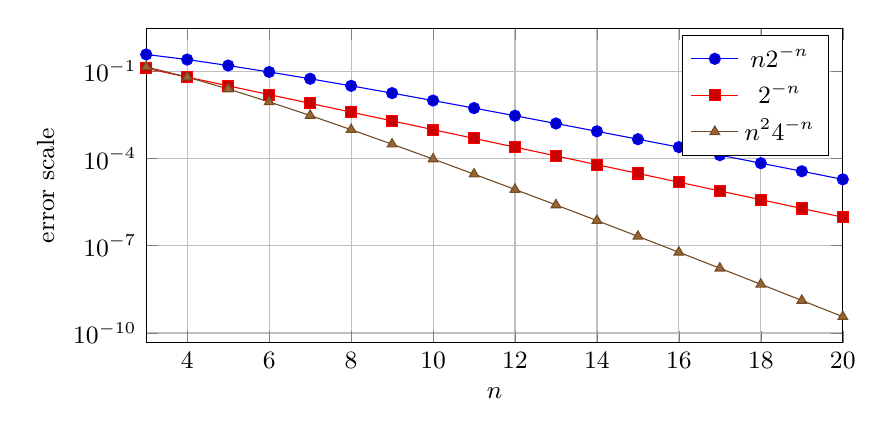
\begin{tikzpicture}
\begin{axis}[
  width=0.86\textwidth,
  height=0.46\textwidth,
  ymode=log,
  xmin=3,xmax=20,
  xlabel={$n$},
  ylabel={error scale},
  grid=both,
  legend style={font=\small,at={(0.98,0.98)},anchor=north east},
  tick label style={font=\small},
  label style={font=\small}
]
\addplot+[mark=*] coordinates {
 (3,0.375) (4,0.25) (5,0.15625) (6,0.09375) (7,0.0546875)
 (8,0.03125) (9,0.017578125) (10,0.009765625) (11,0.00537109375)
 (12,0.0029296875) (13,0.0015869140625) (14,0.0008544921875)
 (15,0.000457763671875) (16,0.000244140625) (17,0.00012969970703125)
 (18,0.00006866455078125) (19,0.0000362396240234375) (20,0.000019073486328125)
};
\addlegendentry{$n2^{-n}$}
\addplot+[mark=square*] coordinates {
 (3,0.125) (4,0.0625) (5,0.03125) (6,0.015625) (7,0.0078125)
 (8,0.00390625) (9,0.001953125) (10,0.0009765625) (11,0.00048828125)
 (12,0.000244140625) (13,0.0001220703125) (14,0.00006103515625)
 (15,0.000030517578125) (16,0.0000152587890625) (17,0.00000762939453125)
 (18,0.000003814697265625) (19,0.0000019073486328125) (20,0.00000095367431640625)
};
\addlegendentry{$2^{-n}$}
\addplot+[mark=triangle*] coordinates {
 (3,0.140625) (4,0.0625) (5,0.0244140625) (6,0.0087890625)
 (7,0.00299072265625) (8,0.0009765625) (9,0.000308990478515625)
 (10,0.000095367431640625) (11,0.0000288486480712890625)
 (12,0.00000858306884765625) (13,0.000002518296241760254)
 (14,0.0000007301568984985352) (15,0.00000020954757928848267)
 (16,0.000000059604644775390625) (17,0.000000016821548342704773)
 (18,0.00000000471482053399086) (19,0.0000000013133103493601084)
 (20,0.0000000003637978807091713)
};
\addlegendentry{$n^2 4^{-n}$}
\end{axis}
\end{tikzpicture}
\caption{The three scales in \eqref{eq:binary-phase-expansion}.  The deterministic
center drift $n2^{-n}$ dominates the one-cell scale $2^{-n}$ and the quadratic
Taylor scale $n^2 4^{-n}$.}
\label{fig:three-scales}
\end{figure}

\section{Exact special values}
\label{sec:special-values}

The general estimates become especially transparent at $0$, $1/2$, and $1$.

\subsection{The endpoints}

Since $a_{n,0}=1$,
\begin{equation}
 \mathcal A_n(0)=2^{-\binom n2}.                            \label{eq:A-zero}
\end{equation}
At $x=1$, the index is $2^n$.  Using
$P_n=P_{n-1}(1+z+\cdots+z^{2^n-1})$ and
$g_{n-1}<2^n$, the coefficient at $z^{2^n}$ is the sum of all coefficients of
$P_{n-1}$ except the constant term.  Thus
\begin{equation}
 \mathcal A_n(1)=1-2^{-\binom n2}.                          \label{eq:A-one}
\end{equation}
Hence
\begin{equation}
 \mathcal A_n(0)-F(0)=2^{-\binom n2},
 \qquad
 \mathcal A_n(1)-F(1)=-2^{-\binom n2}.                     \label{eq:endpoint-errors}
\end{equation}
The endpoint convergence is superexponential in $n$, vastly faster than the
interior $n2^{-n}$ law.

\subsection{An exact midpoint coefficient}

\begin{proposition}[Exact midpoint error]
\label{prop:midpoint-exact}
For every $n\ge2$,
\begin{equation}
 \boxed{\displaystyle
 \mathcal A_n\!\left(\frac12\right)
 =\frac12+\frac{n+2}{2^n}-2^{-\binom n2}.}                 \label{eq:midpoint-exact}
\end{equation}
Consequently
\begin{equation}
 \frac{2^n}{n}
 \left(\mathcal A_n\!\left(\frac12\right)-\frac12\right)
 =1+\frac2n-\frac{2^{n-\binom n2}}{n}.                    \label{eq:midpoint-scaled}
\end{equation}
\end{proposition}

\begin{proof}
Let $b_r=[z^r]P_{n-1}(z)$ and $M=2^{n-1}$.  Since $M<2^n$,
\begin{equation*}
 [z^M]P_n(z)=\sum_{r=0}^{M}b_r.
\end{equation*}
Put $D=g_{n-2}=2^{n-1}-n$ and
$C=P_{n-2}(1)=2^{\binom{n-1}{2}}$.  From
$P_{n-1}=P_{n-2}(1+\cdots+z^{2^{n-1}-1})$, the central coefficients are
\begin{equation*}
 b_{D-1}=C-1,
 \qquad b_D=b_{D+1}=\cdots=b_{2^{n-1}-1}=C,
 \qquad b_{2^{n-1}}=C-1.
\end{equation*}
The polynomial $P_{n-1}$ is symmetric, has degree
$g_{n-1}=2^n-n-1$, and total mass $2^{\binom n2}$.  The interval
$[g_{n-1}-M,M]=[D-1,M]$ is precisely the displayed central block.  Pairing
symmetric coefficients gives
\begin{align*}
 2\sum_{r=0}^{M}b_r
 &=2^{\binom n2}+\sum_{r=D-1}^{M}b_r\\
 &=2^{\binom n2}+(n+2)C-2.
\end{align*}
Divide by $2^{\binom n2}$ and use
$C/2^{\binom n2}=2^{-(n-1)}$.
\end{proof}

\begin{center}
\begin{tabular}{@{}rccc@{}}
\toprule
$n$ & $\mathcal A_n(1/2)-1/2$ & $(2^n/n)(\mathcal A_n(1/2)-1/2)$ & leading value $1+2/n$\\
\midrule
4  & $0.3593750000$ & $1.4375000000$ & $1.5000000000$\\
6  & $0.1249694824$ & $1.3330078125$ & $1.3333333333$\\
8  & $0.0390624963$ & $1.2499998808$ & $1.2500000000$\\
10 & $0.0117187500$ & $1.2000000000$ & $1.2000000000$\\
12 & $0.0034179688$ & $1.1666666667$ & $1.1666666667$\\
14 & $0.0009765625$ & $1.1428571429$ & $1.1428571429$\\
16 & $0.0002746582$ & $1.1250000000$ & $1.1250000000$\\
20 & $0.0000209808$ & $1.1000000000$ & $1.1000000000$\\
\bottomrule
\end{tabular}
\end{center}
The tiny discrepancy from $1+2/n$ is exactly the superexponential last term in
\eqref{eq:midpoint-scaled}.

\section{The corresponding result for Rvachev's bump}
\label{sec:up-rate}

For $0\le t<1$, let
\begin{equation}
 \vartheta_n(t)=\fracpart{2^{n+1}t},
 \qquad
 \Delta_n(t)=\frac{n+2-2\vartheta_n(t)}{2^{n+1}}.          \label{eq:Delta-up}
\end{equation}
Then
\begin{equation}
 \xi_{n,\floor{2^{n+1}t}}=2t-1+\Delta_n(t).                \label{eq:up-center-drift}
\end{equation}
The proof of \cref{thm:second-order-expansion} gives, uniformly for $0\le t<1$,
\begin{align}
 \mathcal J_n(t)
 &=\Up(2t-1)+\Up'(2t-1)\Delta_n(t) \notag\\
 &\quad+\frac12\Up''(2t-1)\Delta_n(t)^2+\rho_n^{\Up}(t), \label{eq:up-second-order}
\end{align}
with the same bound as \eqref{eq:second-order-remainder}.  The right endpoint is
exceptional because the coefficient identity stops one index earlier:
\begin{equation}
 \mathcal J_n(1)=-2^{-\binom n2},
 \qquad \Up(1)=0.                                         \label{eq:J-right-endpoint}
\end{equation}
This exceptional error is negligible on every exponential scale discussed here.

\begin{corollary}[Pointwise and uniform rate for $\Up$]
\label{cor:up-rate}
For fixed $t\in(0,1)$,
\begin{equation}
 \frac{2^n}{n}
 \bigl(\mathcal J_n(t)-\Up(2t-1)\bigr)
 \longrightarrow\frac12\Up'(2t-1).                       \label{eq:up-pointwise-rate}
\end{equation}
At $t=1/2$, both the derivative term and the actual error collapse:
\begin{equation}
 \mathcal J_n(1/2)=1-2^{-\binom n2}.                       \label{eq:J-half}
\end{equation}
Moreover,
\begin{equation}
 \lim_{n\to\infty}\frac{2^n}{n}
 \norm{\mathcal J_n-\Up(2\,\cdot-1)}_{L^\infty[0,1]}=1.  \label{eq:up-uniform-rate}
\end{equation}
\end{corollary}

The uniform lower bound may be read at $t=1/4$, since
$\mathcal J_n(1/4)=\mathcal A_n(1/2)$ and
$\Up(-1/2)=F(1/2)=1/2$.

\section{Rates for the histogram and for recentered interpolation}
\label{sec:other-rates}

The sharp $n2^{-n}$ rate belongs to the particular moving sample
\eqref{eq:A-def}.  It should not be attributed to the coefficient histogram
itself.

\subsection{The step histogram}

Every interior point of a histogram cell lies within $h_n/2$ of its center.
Since $\Up$ is $2$-Lipschitz and the center error is given by
\cref{thm:center-estimate},
\begin{equation}
 \norm{\mathcal W_n-\Up}_\infty
 \le 2^{-n}+
 \left(\frac{4n}{3}+\frac{16}{9}\right)4^{-n}.             \label{eq:histogram-upper}
\end{equation}
The constant in front of $2^{-n}$ is sharp.  Near $y=-1/2$, where
$\Up'(y)=2$, move from a cell center to a point arbitrarily close to the right
edge of the same cell.  The histogram remains constant while $\Up$ rises by
$h_n+o(h_n)$; the center error is $o(h_n)$.  Therefore
\begin{equation}
 \boxed{\displaystyle
 \lim_{n\to\infty}2^n\norm{\mathcal W_n-\Up}_\infty=1.}   \label{eq:histogram-sharp}
\end{equation}
Thus the step representation has the expected one-cell rate $2^{-n}$.

\subsection{Linear interpolation through the true centers}

Extend $w_{n,m}$ by zero for all $m\in\Z$, and let $\mathcal L_n$ be the
piecewise-linear function satisfying
\begin{equation}
 \mathcal L_n(\xi_{n,m})=w_{n,m}
 \qquad(m\in\Z).                                          \label{eq:linear-interpolant}
\end{equation}
Let $I_n\Up$ be the ordinary linear interpolant of the exact values
$\Up(\xi_{n,m})$ on the same mesh.  Convexity of interpolation weights and
\cref{thm:center-estimate} give
\begin{equation*}
 \norm{\mathcal L_n-I_n\Up}_\infty
 \le\left(\frac{4n}{3}+\frac{16}{9}\right)4^{-n}.
\end{equation*}
For a $C^2$ function on a mesh of width $h$, the linear interpolation error is at
most $h^2\norm{f''}_\infty/8$.  Since $\norm{\Up''}_\infty\le8$,
\begin{equation}
 \boxed{\displaystyle
 \norm{\mathcal L_n-\Up}_\infty
 \le\left(\frac{4n}{3}+\frac{25}{9}\right)4^{-n}.}        \label{eq:linear-rate}
\end{equation}
Translating by one gives the same bound for an interpolant of $F$ on $[0,1]$.

This estimate removes both the step error and the deterministic $n/2$-cell
drift.  It is the most direct quantitative evidence that the iterated
Thue--Morse coefficients are intrinsically accurate; the slower floor-sample
rate is a coordinate choice.

\begin{center}
\begin{tabularx}{0.96\textwidth}{@{}l>{\raggedright\arraybackslash}Xl@{}}
\toprule
Approximation & Construction & Uniform scale\\
\midrule
Center values & $w_{n,m}$ compared with $\Up(\xi_{n,m})$ & $\bigO(n4^{-n})$\\
Linear center interpolant & interpolate $(\xi_{n,m},w_{n,m})$ & $\bigO(n4^{-n})$\\
Step histogram & keep $w_{n,m}$ constant on its cell & $\sim2^{-n}$\\
Floor sample for $F$ & read $m=\floor{2^n x}$ without recentering & $\sim n2^{-n}$\\
Centered finite spline & different convolution/CDF scheme in the synthesis & at most $2^{-n}$\\
Literal unshifted prefix grid & use order $n$ rather than $n+1$ & fails at the endpoint\\
\bottomrule
\end{tabularx}
\end{center}

\section{Why the constants take these values}
\label{sec:constants}

The proof contains four constants, each with a transparent origin.

\begin{enumerate}
\item The coefficient curvature constant $32$ is
\begin{equation*}
 4\cdot 2^{\binom{n-2}{2}-\binom n2}=32\,4^{-n}.
\end{equation*}
The factor $4$ counts the four shifted copies of $P_{n-2}$ in
\eqref{eq:second-difference-product}.

\item The discrete variance $n/12+1/9$ consists of $n$ unit-width box jitters,
each of variance $1/12$, plus the variance $1/9$ of the scaled Rvachev tail.

\item The leading displacement is $n2^{-n-1}$.  Multiplication by the maximal
slope $F'(1/2)=2$ gives the uniform leading error $n2^{-n}$ and hence the sharp
constant $1$.

\item The quadratic Taylor coefficient uses the sharp bound
$\norm{F''}_\infty\le8$, while the cubic remainder uses
$\norm{F'''}_\infty\le64$.  These are the $r=2$ and $r=3$ instances of
\eqref{eq:derivative-bounds}, not fitted numerical estimates.
\end{enumerate}

The hierarchy can be summarized schematically as
\begin{equation}
 \underbrace{n2^{-n}}_{\text{degree/center drift}}
 \;\gg\;
 \underbrace{2^{-n}}_{\text{binary floor phase and one-cell error}}
 \;\gg\;
 \underbrace{n^2 4^{-n}}_{\text{quadratic Taylor term}}
 \;\gg\;
 \underbrace{n4^{-n}}_{\text{intrinsic center error}}.     \label{eq:hierarchy}
\end{equation}
For fixed $x$, the first two terms are explicitly visible in
\eqref{eq:binary-phase-expansion}.  The third is the first smooth nonlinear
correction.  The fourth is where the finite coefficient law itself differs from
the infinite Rvachev law.

\section{A Lean formalization roadmap}
\label{sec:lean-roadmap}

The new theorem is well aligned with the current module decomposition.
The existing formalized chain is:
\begin{enumerate}
\item \path{ThueMorsePrefix.lean}: \texttt{iteratedPrefix}, the binomial
      convolution law, Prouhet cancellation, and exact dyadic zero runs;
\item \path{ThueMorseGenerating.lean}: formal power-series identities and the
      corrected normalized grid;
\item \path{ThueMorseApproximation.lean}:
      \path{iteratedPrefix_eq_approximationPolynomial_coeff},
      \path{correctedPrefixCoefficient_eq_stepApproximant}, and the
      qualitative convergence theorems;
\item \path{StepApproximationLimit.lean}: coefficient monotonicity and the
      moving-argument squeeze used for pointwise convergence.
\end{enumerate}

A formal proof of \cref{thm:uniform-rate} can be organized into the following
small additions.

\begin{enumerate}
\item Define the zero-extended normalized coefficient row $w_{n,m}$ on $\Z$ and
      prove \eqref{eq:curvature-bound} by coefficient extraction from
      \eqref{eq:second-difference-product}.  This is algebraic and should require
      no measure theory.

\item Reuse the existing cosine-product theorem to define $q_n$ and prove
      $\Up=\mu_n*q_n$.  The identity \eqref{eq:tail-factorization} is a direct
      reindexing plus the standard infinite cosine product.

\item Prove the cardinal partition
      $\sum_k hq_n(kh)=1$ by factoring one box density.  The center averaging
      identity \eqref{eq:cardinal-average} then follows from convolution with an
      atomic measure.

\item For a first formal rate, use the compact support of $q_n$ and obtain the
      elementary $4(n+2)^2 4^{-n}$ center bound.  This avoids differentiated
      Poisson summation and already proves the sharp $n2^{-n}$ limit.

\item In a second refinement, invoke the repository's Poisson-summation layer to
      prove the exact second moment \eqref{eq:lambda-second-moment}; this upgrades
      the center estimate to \eqref{eq:center-estimate}.

\item Formalize the exact drift identity \eqref{eq:center-drift}, apply the
      repository's derivative bounds, and finish with a uniform Taylor estimate.
      The exact midpoint formula \eqref{eq:midpoint-exact} supplies the matching
      lower bound without any compactness argument.
\end{enumerate}

The logical core of the sharp constant requires only the weaker center estimate.
Thus the project can be split cleanly: first formalize the asymptotic constant
$1$ with elementary support bounds, then strengthen the remainder by adding the
cardinal second-moment calculation.

\section{Conclusion}
\label{sec:conclusion}

The iterated signed Thue--Morse prefixes approach the Fabius function through a
sequence of exact algebraic identifications:
\begin{equation*}
 \text{prefix sums}
 \longleftrightarrow
 \text{coefficients of }P_n
 \longleftrightarrow
 \text{center heights of }\mathcal W_n
 \longrightarrow \Up
 \longrightarrow F.
\end{equation*}
The first two arrows are exact below the first omitted dyadic coefficient.  The
last two were already known qualitatively.  The quantitative analysis shows that
the finite coefficient law is exceptionally accurate at its natural centers:
its error is only $\bigO(n4^{-n})$.  The floor sample used to recover $F$ reads
those centers at a deterministic displacement
\begin{equation*}
 \delta_n(x)=\frac{n}{2^{n+1}}+
 \frac{1-\fracpart{2^n x}}{2^n}.
\end{equation*}
That displacement produces the complete leading behavior.

The final result is therefore both sharp and explanatory:
\begin{equation*}
 \mathcal A_n(x)-F(x)
 =F'(x)\delta_n(x)+\bigO(n^2 4^{-n}),
 \qquad
 \frac{2^n}{n}(\mathcal A_n-F)\longrightarrow\frac12F'
 \quad\text{uniformly}.
\end{equation*}
Moreover
\begin{equation*}
 \norm{\mathcal A_n-F}_\infty
 =(n+2)2^{-n}+\bigO(n^2 4^{-n}).
\end{equation*}
The leading pointwise profile is $F'/2$, the leading uniform constant is $1$,
and the next term remembers the binary tail $\fracpart{2^n x}$.  Recenter
and interpolate the same coefficients, and the factor $n2^{-n}$ disappears,
leaving the much faster explicit bound $\bigO(n4^{-n})$.

\appendix

\section{Notation crosswalk}
\label{app:notation}

\begin{center}
\begin{tabularx}{0.96\textwidth}{@{}l>{\raggedright\arraybackslash}X@{}}
\toprule
Symbol & Meaning\\
\midrule
$\varepsilon_m$ & signed Thue--Morse value $(-1)^{\wt(m)}$\\
$\sigma_k(m)$ & $k$-fold inclusive prefix sum of $\varepsilon_m$\\
$P_n(z)$ & $\prod_{j=1}^n(1+z+\cdots+z^{2^j-1})$\\
$a_{n,m}$ & coefficient $[z^m]P_n(z)$\\
$g_n$ & degree $2^{n+1}-n-2$ of $P_n$\\
$h_n$ & mesh width $2^{-n}$\\
$\xi_{n,m}$ & centered coefficient location $(2m-g_n)/2^{n+1}$\\
$w_{n,m}$ & normalized height $a_{n,m}/2^{\binom n2}$\\
$\mu_n$ & centered atomic coefficient distribution\\
$\mathcal W_n$ & box-smoothed coefficient histogram $\mu_n*\beta_{h_n}$\\
$\mathcal J_n(t)$ & corrected bump sample $\sigma_{n+1}(\floor{2^{n+1}t})/2^{\binom n2}$\\
$\mathcal A_n(x)$ & Fabius sample $\mathcal J_n(x/2)$\\
$\delta_n(x)$ & exact center displacement in \eqref{eq:delta-def}\\
$\theta_n(x)$ & binary phase $\fracpart{2^n x}$\\
$\lambda_{n,k}$ & cardinal tail weights $h_nq_n(kh_n)$\\
\bottomrule
\end{tabularx}
\end{center}

\section{A compact statement of the main estimates}
\label{app:summary}

For rapid reference, for every $n\ge3$:
\begin{align*}
\sup_{m\in\Z}
 \abs{\mathcal W_n(\xi_{n,m})-\Up(\xi_{n,m})}
 &\le\left(\frac{4n}{3}+\frac{16}{9}\right)4^{-n},\\
\norm{\mathcal W_n-\Up}_\infty
 &\le2^{-n}+\left(\frac{4n}{3}+\frac{16}{9}\right)4^{-n},\\
\norm{\mathcal L_n-\Up}_\infty
 &\le\left(\frac{4n}{3}+\frac{25}{9}\right)4^{-n},\\
\sup_{x\in[0,1]}
 \abs{\mathcal A_n(x)-F(x)-F'(x)\delta_n(x)}
 &\le\left(n^2+\frac{16}{3}n+\frac{52}{9}\right)4^{-n},\\
\sup_{x\in[0,1]}
 \abs{\mathcal A_n(x)-F(x)-F'(x)\delta_n(x)
       -\tfrac12F''(x)\delta_n(x)^2}
 &\le\left(\frac{4n}{3}+\frac{16}{9}\right)4^{-n}
      +\frac43(n+2)^3 8^{-n}.
\end{align*}
The normalized profile and norm satisfy
\begin{align*}
 \sup_{x\in[0,1]}
 \abs{\frac{2^n}{n}(\mathcal A_n(x)-F(x))-\frac12F'(x)}
 &\le \frac2n+\left(n+\frac{16}{3}+\frac{52}{9n}\right)2^{-n},\\
 -2^{-\binom n2}
 \le \norm{\mathcal A_n-F}_\infty-(n+2)2^{-n}
 &\le(n+3)^2 4^{-n}.
\end{align*}
The exact asymptotic conclusions are
\begin{align*}
 \frac{2^n}{n}(\mathcal A_n-F)
 &\longrightarrow\frac12F' &&\text{uniformly on }[0,1],\\
 \frac{2^n}{n}\norm{\mathcal A_n-F}_\infty
 &\longrightarrow1,\\
 2^n\norm{\mathcal W_n-\Up}_\infty
 &\longrightarrow1.
\end{align*}

\begin{thebibliography}{99}

\bibitem{fabius1966}
J.~Fabius,
\newblock A probabilistic example of a nowhere analytic $C^\infty$-function,
\newblock \emph{Zeitschrift für Wahrscheinlichkeitstheorie und Verwandte Gebiete}
  \textbf{5} (1966), 173--174.
\newblock DOI: \nolinkurl{10.1007/BF00536652}.

\bibitem{arias1982}
J.~Arias de Reyna,
\newblock Definición y estudio de una función indefinidamente diferenciable de
  soporte compacto,
\newblock \emph{Revista de la Real Academia de Ciencias Exactas, Físicas y
  Naturales de Madrid} \textbf{76} (1982), no.~1, 21--38.
\newblock English translation: \emph{An infinitely differentiable function with
  compact support: Definition and properties}, arXiv:\nolinkurl{1702.05442} (2017).

\bibitem{arias2018}
J.~Arias de Reyna,
\newblock Arithmetic of the Fabius function,
\newblock \emph{INTEGERS} \textbf{18} (2018), Article A51;
  arXiv:\nolinkurl{1702.06487}, version~3.

\bibitem{allouche2003}
J.-P.~Allouche and J.~Shallit,
\newblock \emph{Automatic Sequences: Theory, Applications, Generalizations},
\newblock Cambridge University Press, 2003.

\bibitem{proveit}
V.~Reshetnikov,
\newblock \emph{ProveIt: Analysis/FabiusFunction},
\newblock Lean~4 formal development, main branch studied 25 August 2026.
\newblock \url{https://github.com/VladimirReshetnikov/ProveIt/tree/main/Analysis/FabiusFunction}.

\bibitem{synthesis}
V.~Reshetnikov,
\newblock \emph{The Fabius Function and Rvachev's Up-Function: Exact arithmetic,
  probability, Fourier analysis, and corrected sharp asymptotics},
\newblock repository LaTeX source, snapshot studied 25 August 2026.
\newblock \url{https://github.com/VladimirReshetnikov/ProveIt/blob/main/Analysis/FabiusFunction/docs/Fabius_Function_and_Rvachev_Up/Fabius_Function_and_Rvachev_Up.tex}.

\end{thebibliography}

\end{document}
